\documentclass[draft,linenumbers]{agujournal2018}
\usepackage{apacite}
\usepackage{url}
\linenumbers
\draftfalse


\journalname{Geophysical Research Letters}
\begin{document}

\title{The importance of ice sheet growth and retreat on magmatism and mantle CO$_2$ flux}

\authors{John J.~Armitage\affil{1}, David J.~Ferguson\affil{2}, Kenni D.~Petersen\affil{3}, and Timothy T.~Creyts\affil{4}}

\affiliation{1}{Dynamique des Fluides G{\'e}ologiques, Institut de Physique du Globe de Paris, Paris, France}
\affiliation{2}{School of Earth and Environment, University of Leeds, Leeds, U.K.}
\affiliation{3}{Department of Geoscience, University of Aarhus, Aarhus, Denmark}
\affiliation{4}{Lamont-Doherty Earth Observatory, Columbia University, U.S.A}

\correspondingauthor{John J.$\sim$Armitage}{armitage@ipgp.fr}


\begin{keypoints}
\item We combine a new history of Icelandic ice-cover with a forward model of magma generation.
\item Magmatism is influenced by both the rate of deglaciation and, importantly, the preceding growth of the ice sheet.
\item For our model to be consistent with observations the rate of melt transport must be high.
\end{keypoints}

\begin{abstract}
Climate cycles may significantly affect the eruptive behavior of terrestrial volcanoes due to pressure changes caused by glacial loading, which raises the possibility that climate change may modulate CO$_{2}$ degassing via volcanism. In Iceland, magmatism is likely to have been influenced by glacial activity. To explore if deglaciation therefore impacted CO$_{2}$ flux we coupled a model of glacial loading over the last $\sim$120\,ka to melt generation and transport. We find that a nuanced relationship exists between magmatism and glacial activity. Enhanced CO$_{2}$ degassing happened prior to the main phase of late-Pleistocene deglaciation, and it is sensitive to the duration of the growth of the ice sheet entering into the LGM, as well as the rate of ice loss. Ice sheet growth depresses melting in the upper mantle, creating a delayed pulse of CO$_{2}$ out-gassing as the magmatic system recovers from the effects of loading.
\end{abstract}

\section{Introduction}

Evidence from several tectonic settings indicates that glaciated volcanic systems respond to changing ice volumes \citep{sigvaldason-etal-1992,jull-1996,maclennan-etal-2002,glazner-etal-1999,jellinek-etal-2004,rawson-etal-2016}, and suggests there was a widespread volcanic response to late-Pleistocene ice retreat \citep{huybers-2009}. The most compelling evidence for climate-coupled volcanism comes from Iceland, where changes in early Holocene lava volumes and magma chemistry are consistent with depressurization during glacial unloading \citep{jull-1996,maclennan-etal-2002,sinton-etal-2005}. Magma generation occurs due to pressure-release melting, as the mantle up-wells beneath rift zones. Although the net change in overburden pressures from variations in ice cover are relatively small, the high rates of change associated with glacial activity can produce significant short-term fluctuations in magmatic output \citep{huybers-2009,lund-2011,crowley-etal-2015,burley-2015}. Carbon readily partitions into magmas during partial melting \citep{rosenthal-etal-2015} and is released as CO$_{2}$ gas at lower crustal pressures, making volcanism the primary pathway for transporting carbon from the Earth's mantle to the atmosphere \citep{dasgupta-2010}. Carbon is concentrated in early formed magma and does not enter the melt uniformly over time. Therefore the extent to which glacially driven changes in primary magma generation alter the flux of CO$_{2}$ depends on where in the melting column melt production is enhanced, the rate of melt transport, and the history of ice sheet growth and retreat.

Global data sets of the number of volcanic eruptions throughout the Pleistocene would suggest there is a correlation between climatic change and volcansim \citep{huybers-2009}, yet data resolution makes testing this association difficult. In Iceland there are just over 300 published dated analysis of the Nb composition of Pleistocene lavas. This is arguably the most complete geochemical record within a region that experienced significant Pleistocene deglaciation. In this study we take a new approach, and use a high resolution model of ice sheet history to drive a forward model of melt generation and transport. We predict the change in eruption rates and melt composition as a function of the changing surface load, and also validate the predicted melt porosity against the seismic structure imaged below Iceland. We subsequently explore under what conditions climate and magmatism might be related, and the implications for CO$_{2}$ degassing.

\section{Modelling of Melt Generation and Transport}

To investigate the impact of glacial activity on melt productivity, melt composition, and CO$_{2}$ flux, we used a model of magma generation and transport coupled to a flexural model for the response to change in load due to the ice sheet history (see Supplementary Material). The coupled model consists of a flexural model of the surface displacement due to the changing surface load as the ice sheet changes in thickness. This model of surface displacement is then coupled to either a 1D vertical column or a 2D corner flow model where the flow of the mantle is prescribed at either an upwelling rate of 10 or $20\rm\,mm\,yr^{-1}$, or lateral spreading rate of $10\rm\,mm\,yr^{-1}$. The higher upwelling rate incorporates the possible active effects of the Icelandic mantle plume \citep{maclennan-etal-2001,kokfelt-etal-2003}. The upwelling column is perturbed by the displacement due to loading, where the viscoelastic decay time of the load is set to 1000 yrs. Carbon partitioning into the melt is assumed to be governed by the coefficients derived by \citet{rosenthal-etal-2015}, and the mantle is assumed to be a depleted mix of primitive mantle and MORB. To approximate this depletion we assume a solidus-depletion gradient of $800\rm\,^{\circ}C$ in line with melting experiments on depleted mantle \citep{wasylenki-etal-2003}.

The surface expression of partial melting to glacial loading/unloading is influenced primarily by the rate at which the melt percolates through the mantle \citep{burley-2015}. To constrain the permeability of melt transport, we examined the effects of varying the permeability coefficient on the seismic properties of the mantle produced by our 1-D model. The thermal structure and porosity was converted to S-wave velocities, assuming that melt reduces the velocity by 7.9\,\% per percent porosity \citep{hammond-2000} and including the effects of attenuation \citep{goes-etal-2012}. Recent joint inversion of teleseismic and ambient noise Rayleigh waves in Iceland would suggest that the S-wave velocity is between 4 and $3.8\rm\,km\,s^{-1}$ at depths of 50 to 150\,km \citep{harmon-2016} (Figure \ref{fg:2}). We find that the permeability coefficient needs to be relatively high ($10^{-5}\rm\,m^{2}$) giving a permeability, $k_{\phi} = k_{0}\phi^{3}$, of the order of $10^{-14}\rm\,m^{2}$ ($\phi \approx 0.001$; Figure \ref{fg:2}), because otherwise porosity would be too large and the S-wave velocity would decrease below the observed values. This permeability is an order of magnitude higher than the upper range used to explore how sea-level change might influence mid-ocean ridge (MOR) magmatism \citep{crowley-etal-2015,burley-2015}, and suggests rates of magmatic ascent of the order of $10\rm\,m\,yr^{-1}$. Previously it has been suggested that delays in signal propagation from the zone of partial melting at MORs to the surface might be of the order of a Milankovitch-scale period, 40\,kyr \citep{huybers-2017}. However, the high permeability required to match the seismic observations from Iceland implies a magmatic system that much more rapidly responds to change in melting conditions, which is in agreement with the fast transport rates estimated from U-series isotope studies \citep{elliot-2014}.

\section{Glacial Forcing Throughout the Pleistocene}

Iceland experienced extensive ice-cover during the last glacial period \citep{patton-etal-2017}, with maximum thicknesses in the center of the island of $\sim$ 2km attained by $\sim$23\,ka (Figure \ref{fg:4}a and b). Deglaciation after the LGM occurred at a varying rate, and was discontinuous. For example, a stage of re-advance occurred during the colder climate of the Younger Dryas (11.7-12.9\,ka) \citep{nordahl-2015}. The final phase of deglaciation was particularly rapid, with the main volcanic zones being largely ice free by $\sim$10\,ka (Figure \ref{fg:4}a). The most uncertain period of the glacial history is the pre-LGM growth of the ice sheet. To create the ice sheet histories shown in Figure \ref{fg:4}b and Figure \ref{fg:5}a we calibrated the ice volume since the LGM against the North Greenland Ice Core Project (NGRIP) $\delta^{18}$O record, and Quaternary sea-level curves assuming a linear correlation between these three signals (see Supplementary Material Text S1). We focus on two scenarios: M1, based on the ICE-5G sea-level curves \citep{peltier-2004}, and M2, based on the sea-level curves of \citet{pico-etal-2017} (Figure S2).

We force our melt model with the 120\,ka glacial history after a 5 Myr model wind-up to steady state (model M1, Figure \ref{fg:4}b). The model predicts peaks in magmatic output and CO$_{2}$ flux as pressure changes due to loading and unloading impact the melt production rate (Figure \ref{fg:4}). The response of the magmatic system to changes in ice cover varies depending on the mantle upwelling rate, the rate-of-change in ice sheet thickness, and the prior ice sheet history. Glacial loading suppresses melt production, leading to a decline in magma supply (see Supplementary Material, Figure S3). For example during the period between 35 and 15\,ka, the growth of the ice sheet reduces eruption rates below 5\,km of melt per Myr (Figure \ref{fg:4}c). The recovery from this loading occurs initially in the deepest part of the system as this region is perturbed the least. Recovery is also faster if the mantle upwelling rate is higher, where an upwelling rate of $20\rm\,mm\,yr^{-1}$ is more responsive than the equivalent $10\rm\,mm\,yr^{-1}$ model (Figure \ref{fg:4}b). Higher rates of change in surface loading will impact melt production more strongly such that small magnitude but rapid deglaciation events, for example at $\sim$85\,ka, have a relatively large effect on eruption rates (Figure \ref{fg:4}c).

The impact of deglaciation events is modulated by the upwelling rate of the solid mantle because the upwelling rate controls the background productivity of the melting model. At slower upwelling rates, i.e. $10\rm\,mm\,yr^{-1}$, some periods of deglaciation are not recorded in the flux of magma erupted. An example of this is the warming event at 60\,ka (Figure \ref{fg:4}), where the $10\rm\,mm\,yr^{-1}$ upwelling model produces no response in either the eruption rate or CO$_{2}$ flux. If however upwelling is more rapid, $20\rm\,mm\,yr^{-1}$, then there is a clear pulse in melt eruption rate (Figure \ref{fg:4}). This is because porosity and productivity are so low, that any pulse in melt production does not reach the surface.

Our models indicate that deglaciation-enhanced melt productivity is not only a function of the rate of deglaciation, but is strongly dependent on the preceding glacial history. For example, in the $20\rm\,mm\,yr^{-1}$ upwelling rate model, the largest CO$_{2}$ peak is estimated to occur at $\sim$60\,ka and not during the volumetrically larger magmatic pulse at the end of the Pleistocene (Figure \ref{fg:4}d). This difference is because when the $\sim$60\,ka warming occurred, the melt was enriched in carbon due to the preceding rapid glaciation. Magmas erupted during the Late-Pleistocene pulse were more depleted in carbon compared to those in the 60\,ka event.

\section{Glacial Forcing Through the Latest Pleistocene and Holocene}

There are two distinct late Pleistocene magmatic pulses, separated by the Younger Dryas cold period (Figure \ref{fg:5}a and b). However, for the model M2 ice sheet history there are three pulses in CO$_{2}$ flux at the end of the Pleistocene, due to the faster ice sheet growth entering the LGM from 35 to 25\,ka in this model (Figure \ref{fg:5}a and e). This peak in CO$_{2}$ flux is because the small magnitude but rapid deglaciations after 25\,ka tap melts rich in trace elements including Nb and carbon (Figure \ref{fg:5}c and d).

The observed time series of incompatible trace element concentrations in Icelandic magmas and ice sheet history have been suggested to be strongly associated \citep{jull-1996,gee-etal-1998,maclennan-etal-2002,sinton-etal-2005,eason-etal-2015}. We find that the predicted change in Nb, which behaves in a similar way to C during mantle melting \citep{rosenthal-etal-2015}, from all our models fit within the range of the observations (Figure \ref{fg:5}c). The M2 model gives the strongest signature in Nb concentrations of deglaciation during the end of the Pleistocene, while the signature is more subdued in the M1 ice sheet model (Figure \ref{fg:5}c). The 1D forward model used is highly idealised, and yet the agreement between the observations and model is encouraging, and suggests the compositional change observed in lavas erupted during the late-Pleistocene to early Holocene is due to rapid deglaciation \citep{maclennan-etal-2002,sinton-etal-2005,gee-etal-1998,eason-etal-2015}. This implies that the observed change in melt composition is due to change in ice sheet loading and that the pre-deglaciation volcanism likely released a significant volume of CO$_{2}$ (Figure \ref{fg:5}e).

The 1D column model will underestimate the impact of change in deep melt productivity, as it cannot capture the deep wings of the zone of partial melting. To explore the impact of this we force a series of 1D models with the vertical flow taken from steady state corner flow perturbed by the flexural response of the deglaciation of a 200\,km wide ice sheet. The half spreading rate is assumed to be $10\rm\,mm\,yr^{-1}$, and the mantle potential temperature is $1450\rm\,^{\circ}C$. Melt travels vertically from the zone of partial melting in columns at 0 to 80\,km from the rift axis (Figure \ref{fg:6}). We find that in the central zone, from the ridge centre to 40\,km distance, the trend in Nb and CO$_{2}$ flux is relatively similar, with a reduction in Nb at 15\,ka. At distances greater that 40\,km, a peak in Nb and CO$_{2}$ flux is predicted to occur with an increasing delay compared to the centre of extension (Figure \ref{fg:6}). 

The full solution to the coupled equations of magma dynamics would suggest that melts generated at a distance of up to 60\,km from the centre of extension are advected to the ridge axis \citep{katz-2008}. If all of the melt generated up to 60\,km from the centre of extension is erupted, then the CO$_{2}$ flux is significantly increased during the Holocene due to the addition input of melt from the distal parts of the zone of partial melting (Figure \ref{fg:6}b). Therefore these low productivity and deep regions of the zone of partial melting might be a key exporter of mantle carbon into the atmosphere. However, the range of observed Nb concentrations are relatively similar to the axial concentrations, from within $<$40\,km of the rift centre (Figure \ref{fg:6}). This would suggest that the widest regions of the zone of partial melting are not sampled by the volcanism in the Reykjanes Ridge and Western Volcanic Zone, leading to an estimate of CO$_{2}$ fluxes more in line with the simpler 1D model.

\section{Discussion and Conclusions}

The models imply that the deglaciation beginning at 18\,ka and continuing through the B{\/o}lling warming at 14.8\,ka released substantial quantities of CO$_{2}$ when compared to the last 120\,ka (Figure \ref{fg:5}c and Figure \ref{fg:6}b), and this elevated CO$_{2}$ release was because of the preceding growth of the ice sheet. Volcanism during this time would have taken place in a sub-glacial environment and unsurprisingly does not feature in the post-glacial sub-aerial record. Evidence from sub-glacial volcanic units (tuyas) erupted during this time period \citep{hartley-etal-2016} suggest volumetric and compositional trends consistent with those predicted by our model (Figure \ref{fg:5}c and Figure \ref{fg:6}).

Forcing our model with the long-term 120\,ka ice sheet history produces a periodic fluxing of CO$_{2}$ from Icelandic volcanoes due to ice-loss events over this period, implying a close link between ice dynamics and magmatic out-gassing. The greatest release of CO$_{2}$, however, occurred during the period of ice-loss just before the Younger Dryas ($\sim$14\,ka), and therefore before the largest phase of late-Pleistocene deglaciation (Figure \ref{fg:6}). The concentration of CO$_{2}$ released in this magmatic pulse was enhanced due to the lack of any significant loss of ice volume since $\sim$40\,ka. This created a magmatic system capable of fluxing large volumes of carbon during the initial period of post-LGM deglaciation (both models M1 and M2, Figure \ref{fg:5}e), and such a pulse of atmospheric CO$_{2}$ is thought to be recorded at between 15 and 14\,ka in the EPICA Dome C ice core \citep{kohler-etal-2011}. It is therefore possible that this pulse of CO$_{2}$ bolstered the climate warming, and final phase of deglaciation, that proceeded the Younger Dryas.

The CO$_{2}$ flux due to deglaciation is strongly influenced by the prior ice sheet growth. It is the sustained growth of the Icelandic ice sheet before 25\,ka lead to the significant pulse in volcanism and CO$_{2}$ upon deglaciation at the end of the Pleistocene (Figure \ref{fg:6}). This would imply that while a rapid loss of mass can trigger increased eruptions, the impact on atmospheric CO$_{2}$ concentrations is strongly modulated by the full history of the changing surface load. In effect we cannot conclude that all deglaciation events, or other rapid unloading events due to for example erosion, lead to a large flux of volatile gases into the Earth’s atmosphere. The Earth system is more complex that such simple causality, yet one clear implication is that deglaciation after a prolonged period of ice-house conditions will lead to a significant carbon degassing of the upper mantle.

\section*{Supporting Information}

A detailed discussion of the methodology can be found in the supporting information \citep{andersen-etal-2004,andrews-2008,armitage-etal-g3-2011,clark-etal-2009,geirsdottir-2011,gibson-2010,gurenko-1995,katz-etal-2003,lambeck-2001,lambeck-etal-2014,mckenzie-1991,miller-etal-2014,ribe-1985,scott-1992,shorttle-2011,silbeck-1975,sleep-1976,spiegelman-1996,spratt-2016}.

\acknowledgments
We would like to thank M. A. Mary Gee (The University of Western Australia) for sharing her Nb composition data from the Reykjanes Peninsular, and Tamara Pico (Harvard University) for sharing her sea level curves. John J. Armitage acknowledges funding from an Agence National de la Recherche (France), Acceul de Chercheurs de Haute Niveau, grant “InterRift”. The 1-D melting model is available from \url{https://bitbucket.com/johnjarmitage/melt1d-icesheet/}

\bibliography{../../../../ref.bib}

\clearpage
\pagebreak
\newpage

\begin{figure}
\includegraphics{../figures/version05/supp-figure4.png}
\caption{Profiles of porosity and S-wave seismic velocity for the two model permeabilities of $k_{0} = 10^{-7}\rm\,m^{2}$ black line, and $k_{0} = 10^{-5}\rm\,m^{2}$ red line. (a) Porosity plotted against depth at steady state. (b) S-wave velocity from the joint inversion of teleseismic and ambient noise Rayleigh waves \citep{harmon-2016} and the predicted S-wave profile from the high permeability case. The model includes the addition of the adiabatic gradient, the anharmonic effects from the mineralogy and effects of attenuation \citep{goes-etal-2012}. The dashed line assumes melt has no effect, the solid line includes a 7.9\,\% reduction in $V_{S}$ per percent melt \citep{hammond-2000}. (c) S-wave velocity predictions for the low permeability case.}
\label{fg:2}
\end{figure}

\begin{figure}
\includegraphics[width=14cm]{../figures/version05/figure2.png}
\caption{Response of the model to periodic and observed ice sheet thickness changes of the last 120\,ka. (a) Map of Iceland showing the locations of the volcanic rift zones in orange and the maximum extent of the ice sheet at the last glacial maximum (dashed line). The boxes show the location of the Reykjanes Peninsular (R.~P.) and the Western Volcanic Zone (W.~V.~Z.). (b) The ice sheet thickness predicted from the ice sheet model M1 over the last 120\,ka. (c) Melt eruption rate and (d) carbon flux response to the step change in ice sheet thickness: black line, an upper mantle permeability coefficient of $k_{0} = 10^{-5}\rm\,m^{2}$ and upwelling velocity of $10\rm\,mm\,yr^{-1}$, and blue line, an upwelling velocity of $20\rm\,mm\,yr^{-1}$.}
\label{fg:4}
\end{figure}

\begin{figure}
\includegraphics[width=14cm]{../figures/version05/figure3.png}
\caption{Impact of ice sheet grown and decay on melt eruption and composition over the last 40\,ka. (a) Ice sheet models M1 and M2 taken from the sea-level models of \citet{peltier-2004} and \citet{pico-etal-2017} respectively. (b) Melt eruption rates (in\,km of melt per Myr): blue solid line, ice sheet history 5G for $k_{0} = 10^{-5}\rm\,m^{2}$ with an upwelling rate of $20\rm\,mm\,yr^{-1}$; blue dashed line, M1 for $k_{0} = 10^{-5}\rm\,m^{2}$ with an upwelling rate of $10\rm\,mm\,yr^{-1}$; black solid line, ice sheet history M2 for $k_{0} = 10^{-5}\rm\,m^{2}$ with an upwelling rate of $20\rm\,mm\,yr^{-1}$. The gray region shows estimated eruption rates from geological observations (5) (in km$^2$ of melt per Myr). (c) Observed and predicted Nb concentrations (ppm), observations are from the Reykjanes Peninsula and the Western Volcanic Zone \citep{gee-etal-1998,sinton-etal-2005,eason-etal-2015} and are binned at 2.5\,kyr intervals from 0 to 17.5\,ka and then at 5\,kyr intervals. (d) Predicted variation of in the concentration of carbon (ppm) within the erupted melt. (e) Predicted variation in the flux of CO$_{2}$, assuming that the flux of CO$_{2}$ that Icelandic volcanism covers an area of 30,000\,km$^{2}$, and CO$_{2}$ (ppm) = 3.67 C (ppm) (see Eq.~23 in the Supplementary Material).}
\label{fg:5}
\end{figure}

\begin{figure}
\includegraphics{../figures/version05/figure4.png}
\caption{Impact of glacial history on off-axis and on-axis melting. A series of 1D column melting models forced by the response to deglaciation (ice sheet history model M1) where the mantle flow is of steady state corner flow. (a) Nb concentrations from the centre of extension out to 60\,km from the centre of extension. The mean concentration weighted by the eruption rate is plotted as the thick black line. (b) Predicted CO$_{2}$ flux from the series of vertical melting models. The late-Pleistocene eruptions are typified by tuya magmatism. This will have been the case up until at least $\sim$14\,ka, where either magmatism was suppressed or when eruptions occurred they will have been beneath at least 1\,km of ice-cover \citep{hartley-etal-2016}. The suppressed melting regime will have become carbon rich because the shallow low-C melt production is damped due to the ice-sheet loading. Upon deglaciation there is increased volcansim, which initially taps the melt rich carbon.}
\label{fg:6}
\end{figure}

\end{document}